% CSC 300: Professional Responsibilities
% Dr. Clark Turner

% Two Column Format
\documentclass[11pt]{article}
%this allows us to specify sections to be single or multi column so that things
% like title page and table of contents are single column
\usepackage{multicol}

\usepackage{graphicx}
\usepackage{dblfloatfix}
\usepackage{fixltx2e}

\usepackage{setspace}
\usepackage{url}

%%% PAGE DIMENSIONS
\usepackage{geometry} % to change the page dimensions
\geometry{letterpaper}

\begin{document}

\title{\vfill Maintenance Courses in a Software Engineering Curriculum} %\vfill gives us the black space at the top of the page
\author{
James Pearson \vspace{10pt} \\
CSC 300: Professional Responsibilities  \vspace{10pt} \\
Section 1 \vspace{10pt} \\
Dr. Clark Turner \vspace{10pt} \\
}
%\date{October 22, 2010} %Or use \Today for today's Date
\date{\today}

\maketitle

\vfill  %in combinaion with \newpage this forces the abstract to the bottom of the page
\begin{abstract}
Although software maintenance makes up most of the work a software engineer will do in the workplace, Cal Poly requires Software Engineering undergraduates to take only two courses that cover software maintenance.  Considering this, is it ethical for the Computer Science department to state that the program is designed to produce software professionals?  The ACM's Software Engineering Code of Ethics lists maintenance as one of the primary focuses for a Software Engineer; given this, the department should require a more thorough instruction in the art of software maintenance for Software Engineering students.
\end{abstract}

\thispagestyle{empty} %remove page number from title page
\newpage


%Create a table of contents with all headings of level 3 and above.
%http://en.wikibooks.org/wiki/LaTeX/Document_Structure#Table_of_contents has
%info on customizing the table of contents
\thispagestyle{empty}  %Remove page number from TOC
\tableofcontents

\newpage

%end the 1 column format


%start 2 column format
\begin{multicols}{2}
%Start numbering first page of content as page 1
\setcounter{page}{1}
%%%%%%%%%%%%%%%%%%%%
%%% Known Facts  %%%
%%%%%%%%%%%%%%%%%%%%
\section{Facts}

The Cal Poly catalog states that the Software Engineering undergraduate degree ``prepares students to become software professionals who develop software 
products on time, within budget, and that meet customer requirements''. \cite{catalogDept}  It also says that the program differs from the similar Computer Science undergraduate degree program in four ways, one of which is having ``classes [that] include significant learning in engineering and management areas such as quality assurance, testing, metrics, maintenance, configuration management and interpersonal management skills.'' \cite{catalogDept}

Three courses in the Computer Science department's section of the 2011-13 Cal Poly Catalog have the word ``maintenance'' in their course description. \cite{catalogCourses}  In one of these, CSC 358 Computer System Administration, the reference is to ``system maintenance''. \cite{catalogCourses}  Given the course title and that the course is billed as teaching ``fundamental concepts of Unix system administration'', \cite{catalogCourses} we can conclude that the maintenance described is of an operating system and its components, rather than a single piece of software in which the maintainer is altering code.  Thus, this course is not of relevance to our discussion.

CSC 309's course description refers to ``maintenance of large software systems'', while CSC 406's simply mentions ``software maintenance''. \cite{catalogCourses}

George E. Stark claims that ``maintenance consumes between 60 percent and 80 percent of a typical product's total software lifecycle expenditures''. \cite{stark97}  Girish Parekh says that it is two-thirds of the lifecycle and consumes at least 50 percent of most programmers' time. \cite{parekh}

Andrews and Lutfiyya, while preparing in 1998 for a software maintenance course at the University of Western Ontario, found no courses at other universities in which students performed maintenance activities on legacy software. \cite{andrews} They also found that ``most computer science programs offer[ed] no more than two software engineering course''. \cite{andrews}

%%%%%%%%%%%%%%%%%%%%%%%%%
%%% Research Question %%%
%%%%%%%%%%%%%%%%%%%%%%%%%
\section{Research Question}

Does the Cal Poly Software Engineering program include enough training in software maintenance in CSC 309 and CSC 406?

Cal Poly requires Software Engineering undergraduates to take only two courses whose course descriptions cover software maintenance, and those courses are designed to teach about several other topics as well. \cite{catalogCourses}  However, the ACM Software Engineering code of ethics lists software maintenance as one of the roles of a software engineer \cite{secode}, and studies have shown that software maintenance consumes a large portion of the software life cycle. \cite{stark97} \cite{parekh}

%%%%%%%%%%%%%%%%%%%%%%%%%
%%% Extant Arguments from External Sources %%%
%%%%%%%%%%%%%%%%%%%%%%%%%
\section{Extant Arguments}

\subsection{Arguments For}

Andrews and Lutfiyya found that their software maintenance course ``gave students valuable experience in the qualitatively different task of software maintenance''. \cite{andrews}  Engle, Ford and Korson state that it is ``important for students to have experienced [software maintenance]''. \cite{engle}

\subsection{Arguments Against}

\subsubsection{Difficulty of Classroom Instruction}

Engle, Ford and Korson's project stemmed from a perceived ``difficulty of preparing a software system upon which maintenance can be performed''; their end product consisted of 10,000 lines of Ada code and 9 documents. \cite{engle}

Andrews and Lutfiyya avoided creating a large maintenance-ready system by involving several clients and working on free software projects under the GNU Project.  One student team had both their first and second projects cancelled due to a lack of available time on the part of the client; this meant they had to switch to new projects twice during the term. \cite{andrews}

In addition, Andrews and Lutfiyya faced complications in grading; each group was working on a different project and each had its own goals. \cite{andrews}  Grades could not even be fairly assigned based on the clients' satisfaction, as one group unknowingly implemented a feature that had been previously finished (but without an updated status in the project wiki). \cite{andrews}

Andrews and Lutfiyya also noted issues with finding available projects that would be stable enough that student code would not be irrelevant by the end of the course, yet new enough to be using cutting-edge technologies that the students were enthusiastic about. \cite{andrews}

% Talk about issues with iRobot in 2011 Capstone?

\subsubsection{Cost of a New Course}

\subsubsection{Cost of Increasing Maintenance Coverage in Existing Courses}

%%%%%%%%%%%%%%%%
%%% Analysis %%%
%%%%%%%%%%%%%%%%
\section{Analysis}

\subsection{Applicability of the SE Code}

This paper will use the ACM's Software Engineering Code of Ethics as a basis for evaluating the ethicality of the Computer Science department's course offerings.  Therefore, we must first show that the SE Code may be applied to the department.

The preamble to the Code explicitly states that it applies to those engaged in the education of software engineers:

\begin{quote}
``Software engineers are those who contribute by direct participation or by teaching, to the analysis, specification, design, development, certification, maintenance and testing of software systems''. \cite{secode}
\end{quote}

A few sentences later, it reaffirms this:

\begin{quote}
``The Code contains eight Principles related to the behavior of and decisions made by professional software engineers, including [...] educators''. \cite{secode}
\end{quote}

% SE Code: ``Software engineers are those who contribute by direct participation or by teaching, to the analysis, specification, design, development, certification, maintenance and testing of software systems.''

``The Computer Science Department educates students in the discipline of computer science'' and has an ``educational mission''. \cite{catalogDept}  Although we will make no claim that computer science is the same as software engineering, the department also claims that ``[t]he BS in Software Engineering prepares students to become software professionals''. \cite{catalogDept}  Therefore, the Computer Science department of Cal Poly falls under the educator category of those the SE Code wishes to regulate.

% 1.06. Be fair and avoid deception in all statements, particularly public ones, concerning software or related documents, methods and tools.
% 2.01. Provide service in their areas of competence, being honest and forthright about any limitations of their experience and education.
% 3.01. Strive for high quality, acceptable cost and a reasonable schedule, ensuring significant tradeoffs are clear to and accepted by the employer and the client, and are available for consideration by the user and the public.
% 3.04. Ensure that they are qualified for any project on which they work or propose to work by an appropriate combination of education and training, and experience.
% 3.11. Ensure adequate documentation, including significant problems discovered and solutions adopted, for any project on which they work.
% 3.15 Treat all forms of software maintenance with the same professionalism as new development.
% 5.06. Attract potential software engineers only by full and accurate description of the conditions of employment.
% 5.11. Not ask a software engineer to do anything inconsistent with this Code. (professors as employees, not fully preparing us)
% 6.04. Support, as members of a profession, other software engineers striving to follow this Code.
% 6.07. Be accurate in stating the characteristics of software on which they work, avoiding not only false claims but also claims that might reasonably be supposed to be speculative, vacuous, deceptive, misleading, or doubtful.
% 6.11. Recognize that violations of this Code are inconsistent with being a professional software engineer.
% 7.01. Encourage colleagues to adhere to this Code.
% 7.02. Assist colleagues in professional development.
%   8.01. Further their knowledge of developments in the analysis, specification, design, development, maintenance and testing of software and related documents, together with the management of the development process.
%   8.03. Improve their ability to produce accurate, informative, and well-written documentation.

%\subsection{Adequate Documentation}
%
%Section 3.11 of the SE Code states that a Software Engineer must ``[e]nsure adequate documentation, including significant problems discovered and solutions adopted, for any project on which they work.'' \cite{secode}
%
%The Oxford Dictionaries define ``adequate'' as ``satisfactory or acceptable in quality or quantity''. \cite{definitionAdequate}
%
%Documentation for a software project can take many forms: code comments, identifier names, API docs, user manuals. % Find source! %
%
%\subsubsection{Code Comments}
%
%Programmers new to writing code comments tend to write comments that explain the obvious \cite{sixWays}; not only do these comments not provide any positive value, but they are actually a detriment to the project:
%
%``Comments don't just save time, they cost it. They take time to read, and they spread out the actual code on the screen, so you can have less of it on your monitor to inspect at one time.'' \cite{sixWays}

\subsection{Accurate Descriptions of Employment}

Section 5 of the SE Code states:

\begin{quote}
``those managing or leading software engineers shall ... [a]ttract potential software engineers only by full and accurate description of the conditions of employment.'' \cite{secode}
\end{quote}

\subsubsection{School vs. Employment}

It has been said that students should ``think of school as their job''. \cite{schoolJob}  If students are employees, are the teachers their managers?  Both teachers and managers hand out assignments; both teachers and managers give out grades based on performance. \cite{performanceReview}  This is an artificial construct (the department is not truly an employer to its students, aside from any extra-curricular employments), but it provides a useful mindset from which to evaluate Section 5.06 for the scope of this paper.

In addition to managers, the SE Code says that it applies to those persons who are ``leading software engineers''.  The Computer Science department has set out a list of courses that Software Engineering undergraduate students must take to graduate. \cite{catalogDegree}  In this way, they are leading students down a specified path of instruction in the field of Software Engineering and thus Section 5 of the SE Code applies to them.

Once again considering the ``school is a job'' adage, we can draw parallels between the ``employment'' discussed in section 5.06 and a student's time at a university.

\subsubsection{Accurate Description}

As stated previously, the catalog descriptions of the Software Engineering program state that a graduate will have experienced ``significant learning'' in maintenance activities. \cite{catalogDept}  As ``significant'' means ``sufficiently great or important to be worthy of attention; noteworthy'' \cite{definitionSignificant}, it is difficult to pin down whether or not any student has gotten ``significant learning'' in \emph{anything}, yet we will attempt to do so.

As previously discussed, there are two courses offered by the Computer Science department that we must consider when looking at an undergraduate's education in software maintenance.  These two courses are ``CSC 309 Software Engineering II'' and ``CSC 406 Software Deployment''.

CSC 309 is a ``[c]ontinuation of the software lifecycle. Methods and tools for the implementation, integration, testing and maintenance of large software systems. Software development and test environments. Software quality assurance. Group laboratory project. Technical presentation methods and practice.'' \cite{catalogCourses}

From this description, it appears that software maintenance is one of six core concepts covered in the course (implementation, integration, testing, maintenance, development and test environments, quality assurance).  In the longest quarter of the year at Cal Poly, there are 51 instructional days. \cite{polyCalendar}  Assuming an even spread of topic coverage, that gives less than 9 days of instruction about software maintenance.  In reality, the number is even less, since the course is usually taught for 2 or 3 days a week. \cite{309Schedule}

CSC 406 covers ``[d]eployment of a sizeable software product by a student team. Software maintenance and deployment economic issues. Management of deployed  software: version control, defect tracking and technical support.'' \cite{catalogCourses}  Again, we see that software maintenance is one of six primary topics addressed in a course taught three days a week. \cite{406Schedule}

With only 30 Monday-Wednesday-Friday instructional days in the quarter \cite{polyCalendar}, a Software Engineering student will receive approximately 10 days of instruction in software maintenance over the course of their academic career.  When compared to the total number of years spent at Cal Poly, this number does not appear to be ``noteworthy''.

\begin{figure*}[tb!]
  \caption{Percentage of time spent on maintenance in CPE 309 and CPE 406 (approximate).}
  \centering
    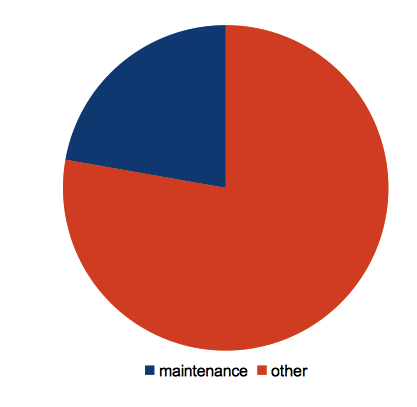
\includegraphics[width=0.5\textwidth]{termpaper/images/pie-chart-01}
\end{figure*}

\begin{figure*}[tb!]
  \caption{Percentage of time spent on maintenance in Software Engineering major courses (approximate).}
  \centering
    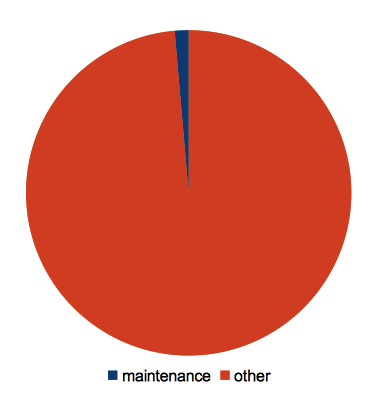
\includegraphics[width=0.5\textwidth]{termpaper/images/pie-chart-02}
\end{figure*}

\begin{figure*}[tb!]
  \caption{Percentage of time spent on maintenance in Software Engineering all courses (approximate).}
  \centering
    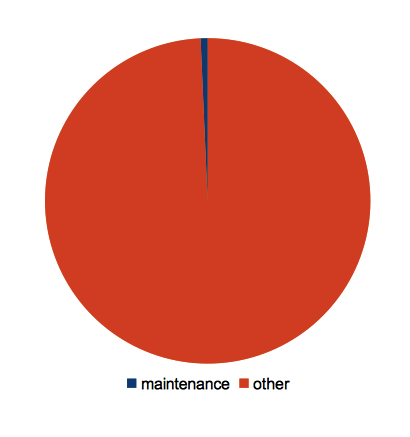
\includegraphics[width=0.5\textwidth]{termpaper/images/pie-chart-03}
\end{figure*}

Thus, the department is not accurate in stating that Software Engineering students experience ``significant learning'' in software maintenance.

\subsubsection{Ethical Analysis}

If we can consider the Computer Science department to be equivalent to a student's manager or leader and the term of their enrollment to be employment, the department violates section 5.06 of the Software Engineering Code of Ethics by not accurately representing the amount of software maintenance done by students in the Software Engineering program.


%\subsection{Avoid Deception in Public Statements}
%
%Section 1.06 of the Code states that a professional Software Engineer must
%
%\begin{quote}
%Be fair and avoid deception in all statements, particularly public ones, concerning software or related documents, methods and tools.\cite{secode}
%\end{quote}
%
%\subsubsection{Public Statements}



%%%%%%%%%%%%%%%%
%%% Conclusion %%%
%%%%%%%%%%%%%%%%
\section{Conclusion}

%end the two column format
\end{multicols}
\newpage

%cite all the references from the bibtex you haven't explicitly cited
\nocite{*}

\bibliographystyle{termpaper/IEEEannot}

\bibliography{termpaper/texreport}

\end{document}
